
\documentclass[12pt]{article}


\usepackage{sbc-template}


\usepackage{graphicx,url}




\usepackage[brazil]{babel}
\usepackage[utf8x]{inputenc}
\usepackage{url}  % para usar URLs nas referencias




\sloppy




\title{Automação de Testes em Aplicações de BPM:\\ um Relato de Experiência}


\author{Jessica Lasch de Moura\inst{1},
Andrea Schwertner Charão\inst{1},\\ Patrícia Pitthan Barcelos\inst{1}, Benhur de Oliveira Stein\inst{1}}
\address{Núcleo de Ciência da Computação\\
Universidade Federal de Santa Maria -- UFSM
\email{\{jmoura, andrea, pitthan, benhur\}@inf.ufsm.br}}




\begin{document}


\maketitle




\begin{resumo}
Este artigo aborda questões relacionadas ao teste automatizado de aplicações desenvolvidas com o apoio de sistemas de gestão de processos de negócio (Business Process Management Systems -- BPMS). Para isso, apresenta-se um relato de experiência de automação de testes de carga e de testes funcionais em uma aplicação de BPM, utilizando-se as ferramentas de código-aberto Apache JMeter e Selenium. A aplicação BPM é baseada na ferramenta Bonita Open Solution (BOS) e encontra-se implantada em uma instituição pública de ensino. Os resultados evidenciam limitações e oportunidades na automação de testes de aplicações de BPM.
\end{resumo}




\begin{abstract}
This article discusses the automated testing of applications developed with the support of Business Process Management Systems -- BPMS. We present an experience report on the automation of load tests and functional tests over a real BPM application, using the Apache JMeter and Selenium open-source tools. The application is developed with a BPM suite named Bonita Open Solution (BOS) and is located in a public educational institution. Results show the limitations and opportunities in test automation of BPM applications.
\end{abstract}




\section{Introdução}
%BPM + teste
A gestão de processos de negócio (\emph{Business Process Management} -- BPM) tem suscitado o interesse da indústria e da academia, tanto por seus benefícios como por seus desafios. Designa-se por BPM o conjunto de conceitos, métodos e técnicas para suportar a modelagem, administração, configuração e análise de processos de negócio~\cite{weske}. Associados a isso, surgiram os sistemas BPM (\emph{Business Process Management Systems} ou \emph{Suites} -- BPMS), que são ferramentas de software para apoio ao ciclo de vida da gestão de processos de negócio. 
%Tais ferramentas têm o potencial de alavancar aumentos de produtividade e redução de custos nos mais variados tipos de organizações.


Dentre os diversos BPMS disponíveis atualmente, é comum encontrar ferramentas com suporte a modelagem, configuração e execução de processos de negócio. Por outro lado, o suporte a tarefas de simulação, monitoramento, verificação e testes ainda é considerado um desafio nesta área~\cite{aalst2013survey}, embora seja determinante para a qualidade do software produzido.  Em particular, o teste automatizado de aplicações de BPM é pouco abordado, tanto pela comunidade da área de BPM~\cite{aalst2013survey} como da área de testes de software~\cite{graham2012experiences}. Diante disso, estima-se que muitas organizações se limitem a testes manuais em suas aplicações de BPM. No entanto, a falta de automação nos testes pode levar a vários problemas durante a implementação e execução de processos de negócio, como baixa aderência aos requisitos, maior esforço dos desenvolvedores, desperdício de tempo e aumento do risco de duplicação de esforços e de erro humano.

%Monitoramento: Business Artifact-Centric Modeling for Real-Time Performance Monitoring
%Verificação:
%Aligning Event Logs and Declarative Process Models for Conformance Checking.
%Massimiliano De Leoni, Fabrizio Maria Maggi and Wil van der Aalst
%Context-Aware Compliance Checking.
%Jan Martijn Van Der Werf, Eric Verbeek and Wil Van Der Aalst
%Where Did I Misbehave? Diagnostic Information in Compliance ...
%Por serem relativamente recentes, os BPMS e a própria tecnologia BPM são pouco desenvolvidos, muitas ferramentas não possuem todas as funcionalidades como modelagem, execução, implantação, simulação e, principalmente,  teste.
%Ainda, gerenciar os dados gerados durante o teste dos processos, de uma forma prática, torna-se uma tarefa difícil.

Nesse contexto, o presente artigo relata uma experiência de automação de testes em uma aplicação de BPM desenvolvida para agilizar um processo em uma instituição pública de ensino. Todas as etapas do desenvolvimento da aplicação, utilizando o BPMS Bonita Open Solution (BOS), foram apresentadas em um trabalho precedente~\cite{sbsi2013}. 
%Os artefatos produzidos neste trabalho foram disponibilizados em um repositório público e a aplicação foi implantada na Universidade Federal de Santa Maria. 
Neste trabalho anterior, as atividades de teste do software foram realizadas manualmente e consumiram um esforço considerável. Mesmo assim, durante a implantação, evidenciou-se alguns defeitos relacionados ao desempenho e a funcionalidades do sistema. Assim, surgiu a motivação para explorar alternativas de automação de testes, visando aumentar a qualidade do software desenvolvido.


O artigo está organizado como segue: a Seção 2 apresenta brevemente alguns conceitos sobre BPM e tecnologias relacionadas, teste de software e sobre como esses tópicos se relacionam. Na sequência, a Seção 3 descreve o processo alvo das experiências e a aplicação construída no trabalho precedente. As seções 4 e 5 apresentam os testes realizados, incluindo a seleção de ferramentas e os resultados obtidos. A Seção 6 comenta trabalhos relacionados e é seguida da Seção 7, que faz as considerações finais e sugere trabalhos futuros.


\section{BPM e Testes}


%\subsection{BPM e suas Tecnologias}


% bpm interdisciplinar
% ciclo bpm
% bpms
% citar grandes players em bpms


A área de BPM pode ser considerada interdisciplinar e, em muitos casos, o termo BPM pode ser usado com significados diferentes~\cite{acmxrds2009}, às vezes com mais ênfase em tecnologia (software) e outras vezes mais associado a gestão. Mesmo assim, a área tem convergido sobre o ciclo de vida de aplicações de BPM, que envolve as atividades de análise, modelagem, execução, monitoramento e otimização~\cite{ABPMP}. 

%Para a etapa de modelagem,  Outro exemplo é a ampla adoção do padrão chamado \emph{Business Process Model and Notation} (BPMN)~\cite{BPMN}, para modelagem de processos.

%Os sistemas de BPM (BPMS) têm se afirmado como ferramentas essenciais para suporte a atividades desse ciclo de vida. Atualmente, pode-se dizer que um típico BPMS oferece recursos para definição e modelagem gráfica de processos, controle da execução e monitoramento de atividades dos processos. Alguns exemplos de BPMS que se destacam neste cenário são IBM Websphere ~\cite{WEBSPHERE}, Oracle BPM Suite~\cite{ORACLEBPM}, Intalio~\cite{INTALIO}, Bizagi~\cite{BIZAGI}, TIBCO BPM~\cite{TIBCOBPM}, Activiti~\cite{ACTIVITI} e Bonita Open Solution ~\cite{BONITASOFT}.

% Referencias acima foram retiradas por ocuparem muito espaco no final. Podem ser substituidas por notas de rodape, caso haja espaco.
Os sistemas de BPM (BPMS) têm se afirmado como ferramentas essenciais para suporte a atividades desse ciclo de vida. Atualmente, pode-se dizer que um típico BPMS oferece recursos para definição e modelagem gráfica de processos, controle da execução e monitoramento de atividades dos processos. Alguns exemplos de BPMS que se destacam neste cenário são IBM Websphere, Oracle BPM Suite, Intalio, Bizagi, TIBCO BPM, Activiti e Bonita Open Solution.

%Em se tratando de software, os sistemas BPM (BPMS) têm se afirmado como ferramentas essenciais para o sucesso de aplicações de BPM. A área tem evoluído rapidamente, levando a diferentes conceituações e classificações de ferramentas no mercado~\cite{gartner, greenresearch, forrester}. 


Nota-se que a preocupação com testes não fica evidente em BPMS. De fato, analisando-se o material promocional e a documentação publicamente disponível sobre os principais BPMS, observa-se uma ênfase em etapas de modelagem e execução. Visivelmente, tais recursos são um diferencial no desenvolvimento de aplicações de BPM, em comparação ao desenvolvimento de software em geral. No entanto, aplicações de BPM também estão sujeitas a defeitos e, por isso, podem se beneficiar de avanços na área de testes de software.

%http://www.researchmoz.us/business-process-management-bpm-cloud-mobile-and-patterns-market-shares-strategies-and-forecasts-worldwide-2013-to-2019-report.html#6161


%melhoria do processo. Alguns exemplos de ferramentas BPMS são Intalio, TIBCO BPM,
%além das soluções Oracle e IBM WebSphere para BPM.
% Existem também ferramentas distribuídas como software livre, tais como Activiti, jBPM, ProcessMaker e Bonita Open Solution.


%\subsection{Testes de Software}
%- teste de software: generalidades
%Em linhas gerais, pode-se dizer que o objetivo dos testes é encontrar defeitos. Desta forma os testes são conduzidos para demonstrar a ausência de qualidade expressa pela presença de defeitos, para tal se faz necessário um processo (planejamento, especificação, execução, análise de resultados), considerando-se sempre os riscos do negócio e a qualidade do produto \cite{pol2002software}.

%-teste de software: tipos de teste
%Em engenharia de software, o teste é tradicionalmente considerado uma prática importante~\cite{pressman, swebok}. Há uma vasta terminologia relacionada a testes de software, classificando-os de acordo com diferentes critérios (objetivos, técnicas, entre outros). Por exemplo, os testes podem abranger o sistema inteiro (teste de sistema), alguns componentes (teste de integração) ou unidades isoladas (teste unitários). Alguns autores também distinguem testes funcionais, que avaliam o comportamento do software frente a seus requisitos, dos testes ditos não-funcionais, que verificam atributos relacionados aos requisitos não-funcionais do software, como por exemplo desempenho e usabilidade~\cite{desikan2006software}. Técnicas de teste podem variar de acordo com a natureza da aplicação~\cite{swebok}, por exemplo: orientada a objetos, baseada na Web, com interface gráfica, etc.
% citar livro do Cem Kaner
% testes de aceitação


Em testes de software, há muitas tarefas que podem ser trabalhosas e propensas a erros quando realizadas manualmente. Por este fato, vários autores relatam a importância dos testes automatizados em ambientes de desenvolvimento~\cite{sbqs2013}. Com a evolução das áreas de qualidade e teste de software, foi surgindo uma variedade de soluções para automação de testes. Ferramentas para testes unitários, por exemplo, são numerosas e costumam se integrar aos ambientes de desenvolvimento~\cite{unittesting}. Outro exemplo é o teste de aplicações baseadas em interfaces gráficas ou Web~\cite{webtesting}.

% vários autores relatam a importância dos testes automatizados dentro de um ambiente de desenvolvimento No artigo Especificação e Automação Colaborativas de Testes utilizando a técnica BDD \cite{sbqs2013}, é abordada a importância de testes automatizados dentro de um ambiente de desenvolvimento e os autores utilizam a ferramenta Selenium Webdriver.


%http://en.wikipedia.org/wiki/List_of_GUI_testing_tools


%Pressman define quatro tipos de teste de software: teste de unidade, teste de integração, teste de validação, teste de sistema. Teste de unidade concentra-se em cada unidade do software, de acordo com o que é implementado no código fonte, utiliza as técnicas de teste de caixa branca e caixa preta. Teste de integração concentra-se no projeto e na construção da arquitetura de software, utilizando principalmente as técnicas de teste de caixa preta. No teste de validação os requisitos estabelecidos como parte da análise de requisitos de software são validados em relação ao software que foi construído. Por último, no teste de sistema, o software e outros elementos do sistema são testados como um todo. Teste de segurança e recuperação \cite{pressman1995engenharia}. O teste de sistema pode ser dividido em uma série de diferentes testes, cujo objetivo principal é por completamente à prova o sistema, dentre estes sub-tipos de testes está o teste de carga.


%O teste de carga executa o sistema de uma forma que exige recursos em grande quantidade como, por exemplo, simular um grande número de acessos simultâneos em um determinado servidor num horário de pico. O teste de carga permite identificar a que ponto o sistema deixa de responder ou deixa de responder em um tempo adequado.


%\subsection{Testes em Aplicações de BPM}


%Embora o termo ``teste'' não seja frequente na literatura sobre BPM, o ciclo de vida de aplicações de BPM inclui as etapas de monitoramento e otimização, que se dedicam a identificar e corrigir problemas~\cite{weske}. Tal visão do ciclo de vida é comumente voltada a aspectos de gestão, não de tecnologia (software). Mesmo assim, acreditamos que o teste de software relacione-se particularmente com essas etapas e, de forma geral, possa contribuir significativamente para o sucesso de aplicações de BPM.


Aplicações de BPM podem ser tratadas como software em geral. Assim, é possível testá-las sob diferentes aspectos, por meio de tipos de testes já consagrados em engenharia de software, como por exemplo testes funcionais do tipo caixa-preta ou teste de carga. Sob esta ótica, pode-se empregar ferramentas de automação de testes alinhadas com cada tipo de teste. No entanto, a adoção esta abordagem pode ter limitações e dificuldades, pois não leva explicitamente em conta o ciclo de vida de aplicações de BPM.
% testes de aceitação

%Há alguns anos, o termo \emph{Business Process Testing -- BPT} vem sendo empregado para designar testes de processos de negócio. Não há uma caracterização clara deste tipo de teste, sendo que em alguns contextos o termo refere-se a testes automatizados reusáveis criados por especialistas do domínio~\cite{hp}, portanto aderentes aos processos de negócio. Em outros contextos, o termo relaciona-se a automação de testes de processos implementados em arquiteturas orientadas a serviços (\emph{Service Oriented Architectures} -- SOA)~\cite{soatest2008, bpeltest2008}. Testes deste tipo possuem uma relação com BPM e são uma especialização de testes de software em geral. No entanto, pode-se dizer que essa relação com BPM é fraca, pois é principalmente focada na etapa de execução dos processos. Além disso, não costumam ser soluções integradas em sistemas BPM.


% sistemas BPMS: simulação, monitoramento...
%http://www8.hp.com/us/en/software-solutions/software.html?compURI=1174789#.UvTvdfjei1H


%Aspectos comuns a qualquer tipo de software
%- verificação (conformidade, corretude, ...)


%Aspectos particulares
%- verificação dos modelos BPMN
%- caminhos críticos e gargalos (simulação)


%Os desafios da homologação de Processos Automatizados
%http://blog.iprocess.com.br/2013/04/os-desafios-da-homologacao-de-processos-automatizados/


\section{Processo Alvo dos Testes}
%- o nosso caso: processo,
Os testes realizados neste trabalho referem-se a um processo realizado com frequência em instituições de ensino superior, que é a apreciação de Atividades Complementares de Graduação (ACGs), ou seja, atividades que formam a parte flexível do currículo dos graduandos (participação em palestras, eventos, projetos, etc.). Em um trabalho anterior~\cite{sbsi2013}, aplicou-se BPM a este processo, visando agilizar a apreciação de ACGs em um curso de graduação da Universidade Federal de Santa Maria. Desenvolveu-se assim uma aplicação de BPM que foi colocada em produção, passando pelas etapas de análise, modelagem, execução e monitoramento, com o apoio da ferramenta Bonita Open Solution (BOS)~\footnote{Atualmente distribuída sob o nome Bonita BPM}.


Bonita Open Solution (BOS)~\cite{BONITASOFT} é um BPMS desenvolvido em Java, pela empresa BonitaSoft, distribuído sob uma licença de software livre. A ferramenta oferece componentes tanto para a modelagem como para a execução e monitoramento de processos, numa abordagem integrada. 
%É possível agregar funcionalidades às aplicações através de conectores (por exemplo, para conexão com banco de dados, envio de emails, geração de relatórios, etc.). Também é possível desenvolver novos conectores e extensões utilizando a linguagem Groovy. 
A escolha do BOS deu-se principalmente por ser um software livre com reconhecimento no mercado, capaz de atender alguns requisitos específicos da aplicação (em particular, integração com base de usuários LDAP existente e com sistema de gerenciamento de documentos).


No processo implementado, há 12 atividades, distribuídas entre 5 divisões de responsabilidade (papéis de aluno, professor orientador, relator, colegiado e coordenação do curso)~\cite{sbsi2013}. Também há formulários Web relativos a cada divisão de responsabilidade. No início do processo, o aluno preenche um formulário e o submete a apreciação, anexando os documentos comprobatórios da atividade (certificados e atestados, por exemplo). De acordo com o tipo de atividade, o fluxo é direcionado para os responsáveis pela avaliação e validação da ACG (professores, membros do colegiado e secretaria do curso).


A aplicação implementada passou por testes funcionais realizados manualmente, além de testes de aceitação realizados com um pequeno grupo de usuários reais. Após algumas semanas em operação, a aplicação revelou problemas como, por exemplo, instâncias que falharam devido a entradas inesperadas, serviços que não foram restabelecidos corretamente após serem interrompidos e, inclusive, congestionamentos devido ao grande número de casos abertos numa data limite, estipulada pelo colegiado do curso. Este último problema, em particular, culminou com uma demora excessiva na carga dos formulários Web, levando à decisão de interromper a operação do sistema para investigação. Essa experiência evidenciou que testes podem ser determinantes para o sucesso de uma aplicação de BPM. A partir disso, surgiu a motivação para buscar soluções para automatização de testes com o processo.


%alterado
No planejamento dos testes automatizados, priorizou-se o teste de  etapas que de fato revelaram problemas durante a operação. Com isso, buscou-se verificar se os problemas poderiam ser facilmente identificados antes de colocar-se a aplicação em produção. Os testes escolhidos foram: (a) testes de carga, que são um tipo de teste de desempenho, visando avaliar o comportamento do sistema frente a um grande número de solicitações e (b) testes funcionais, a fim de verificar as saídas do sistema produzidas a partir de entradas pré-definidas. \textbf{Nenhum destes tipos de teste possui suporte no BPMS utilizado} (Bonita Open Solution), que inclui somente funcionalidades limitadas de simulação e depuração de execução dos processos. Assim, realizou-se um levantamento de ferramentas de teste disponíveis e selecionou-se as mais promissoras, antes de partir-se para o detalhamento e execução dos testes, conforme descrito nas seções seguintes.
% As seções seguintes descrevem as experiências com cada tipo de teste.




%- planos de teste


\section{Testes de Carga}


%\subsection{Seleção de Ferramentas}\label{s:loadtools}
%*visão geral da ferramenta, relação com testes-BPM, justificativa para escolha (de %preferência, argumentos que se apliquem a outros casos)


%outras opções de ferramentas
%Existem diversas ferramentas para automação de testes, especificamente se tratando de testes de carga e desempenho existem duas ferramentas próximas ao JMeter que são o The Grinder e o WebLOAD, ambas são ferramentas open source e tem diversas funcionalidades. No entanto, a maior desvantagem dessas ferramentas é que não existe a possibilidade de capturar as requisições que devemos testar de uma forma automática, todas requisiçõesp recisam ser inseridas manualmente no plano de teste. No JMeter existe a opção 'Servidor de Proxy' que permite capturar o tráfico de requisições e este é automaticamente transformado em requisições no plano de teste.


%Considerando que a aplicação desenvolvida é operada por meio de um navegador Web, é possível realizar testes de carga com o apoio de ferramentas voltadas para aplicações Web. Neste caso, consegue-se testar o desempenho conjunto de toda a pilha de software do sistema, desde o sistema operacional até os servidores de aplicações Web e banco de dados, incluindo o motor de execução dos processos. 
%Também seria possível aplicar testes de carga nos componentes em separado, mas esta opção pareceu-nos mais limitada em um primeiro momento.


Dentre as diversas ferramentas disponíveis para testes de carga em aplicações Web, pode-se citar HP LoadRunner, IBM Rational Performance Tester e Neotys Neoload, que são comercializadas; Apache JMeter, Curl-loader e Gatling, que são software livre e gratuito; e também plataformas de teste em nuvem, como por exemplo Blitz e LoadStorm, que oferecem o serviço com planos de precificação variados. Dentre essas, deu-se preferência à ferramenta JMeter, por ser software livre com grande comunidade de usuários e vasta documentação.

% ferramentas livres, com grande comunidade de usuários, pois no contexto do trabalho (instituição pública) seria injustificável escolher uma ferramenta comercial com alternativa livre. A ferramenta Apache JMeter é bastante citada em fóruns técnicos e possui vasta documentação, por isso foi escolhida para este trabalho. 
%Esta ferramenta também é citada no contexto específico de aplicações de BPM~\cite{infosys}.


%Apache JMeter é uma ferramenta para desktop, desenvolvida em Java, voltada para testes de desempenho de aplicações Web.  JMeter pode ser usado para testar o desempenho tanto em recursos estáticos quanto dinâmicos (arquivos, linguagens dinâmicas da Web - PHP, Java, ASP.NET, etc -, objetos Java, bases de dados, servidores FTP, entre outros). Ele pode simular um teste de carga em um servidor, grupo de servidores, rede ou objeto para testar a sua capacidade ou para analisar o desempenho global em diferentes tipos de carga~\cite{JMeter}.


%relação com bpm e justificativa:
%A escolha da ferramenta JMeter para testar aplicações BPM deu-se por diversos motivos. Primeiramente, pelo fato de o JMeter ser uma ferramenta independente de plataformas e isto é importante pois aplicações baseadas na tecnologia BPM comumente estão hospedados em servidores com os mais diversos sistemas operacionais. O JMeter também permite a criação de diversos usuários para a execução dos testes e aplicações BPM precisam ser testadas com vários usuários, tanto em empresas em que o número de usuários do sistema cresce com o tempo ou, como no nosso exemplo, vários usuários podem iniciar um processo ao mesmo tempo (para solicitar uma 
). Ainda, um fato importante tanto para empresas e quanto para estudo, é uma ferramenta gratuita.


\subsection{Descrição dos Testes}


%escolha do que testar
%etapas de preparação do teste
%ambiente do teste

Para definir a cobertura dos testes de carga, buscou-se identificar as etapas críticas do processo, em que o sistema recebe requisições Web em maior quantidade e tamanho. No caso em questão, o ponto mais crítico é a primeira atividade, em que o aluno preenche um formulário e anexa um comprovante para solicitar aproveitamento da ACG em seu histórico escolar. Assim, decidiu-se limitar o teste de carga a essa atividade.

%Assim, pode-se dizer que a primeira atividade é a etapa mais crítica de todo o processo, 

%No processo em questão, a primeira etapa é onde o usuário (aluno) preenche um formulário e anexa um comprovante para solicitar aproveitamento da atividade em seu histórico escolar. O número de alunos (cerca de 180) é superior ao número de professores, além disso cada aluno geralmente possui várias atividades para solicitar ao final de cada semestre letivo. Após a solicitação do aluno, o processo pode seguir diferentes rotas, algumas mais curtas que outras. Além disso, em algumas divisões de responsabilidade (colegiado, coordenação), os papéis podem ser desempenhados alternativamente por diferentes usuários, evitando possíveis gargalos. 


Um teste de carga com JMeter organiza-se em várias etapas. Na primeira delas, é necessário identificar as requisições Web enviadas ao servidor de aplicação. De posse desses dados, configura-se um plano de teste (script) com vários elementos, por exemplo: grupos de usuários virtuais (que se relacionam à quantidade de requisições simultâneas ao sistema), requisições e ações de pré e pós-processamento destas. A etapa seguinte diz respeito à execução do teste propriamente dito. Os resultados podem ser visualizados durante e após a execução, de diferentes formas (gráficos, tabelas, etc.).


Para identificar as requisições Web enviadas ao servidor (Apache Tomcat com BOS e a aplicação BPM instalados), foi necessário capturar e interpretar o tráfego entre o navegador e o servidor Web. Esta etapa consumiu um tempo considerável, empregando-se diferentes ferramentas (Firebug, Fiddler, BlazeMeter e servidor proxy do JMeter), até se conseguir reproduzir as requisições. A maior dificuldade foi com relação a requisições Web geradas com o Google Web Toolkit (GWT), utilizado internamente pelo Bonita Open Solution.
Notou-se que o teste de aplicações com GWT utilizando o JMeter é um problema frequente em fóruns técnicos, pois há poucas ferramentas capazes de interpretar requisições do tipo GWT-RPC para reprodução no JMeter. Em nosso caso, obteve-se sucesso por meio do uso combinado do servidor proxy do JMeter, com seu recurso de visualização do cabeçalho das requisições, e com o BlazeMeter Chrome Extension, um plugin para o navegador Google Chrome.


%pode-se empregar ferramentas clássicas para desenvolvedores Web. Assim, uma primeira escolha foi o plugin para navegador Firebug~\cite{FIREBUG}, por ser uma ferramenta já disponível no ambiente de desenvolvimento. Com esta ferramenta, conseguiu-se capturar as requisições de login e autenticação de usuário e envio da primeira parte do formulário de solicitação (o formulário é composto de duas partes). No entanto, após estas requisições, o Firebug não foi mais capaz de interpretar o tráfego Web.


%A fim de obter mais informações sobre o tráfego entre o navegador e o servidor Web, utilizou-se então uma funcionalidade da ferramenta JMeter, que permite criar um servidor proxy HTTP para capturar requisições. Utilizando isso, foi possível capturar melhor o tráfego, incluindo etapas que foram omitidas durante a captura com a ferramenta Firebug. No entanto, ao executar o teste utilizando as requisições produzidas através do servidor proxy, algumas etapas do teste apresentaram erros cuja razão não ficou evidente. Com o objetivo de esclarecer e solucionar os erros, decidiu-se usar uma terceira ferramenta para captura do tráfego de dados, Fiddler~\cite{FIDDLER}, que é bastante popular e muito utilizada para efetuar este tipo de captura ~\cite{lawrence2012debugging}.

%Também utilizando o servidor proxy, não é necessário criar cada requisição equivalente no JMeter, pois estas são criadas automaticamente.


%Com os dados coletados através do Fiddler, foi possível verificar que estes eram muito semelhantes aos coletados via o servidor proxy do JMeter e, inclusive, mostravam erros de execução nos mesmos pontos. Assim, foi necessário aprofundar o estudo sobre as requisições HTTP, avaliando sua estrutura, valores esperados, entre outras informações. Com esse estudo foi possível verificar que todas as requisições que apresentavam erro na execução do teste possuíam uma característica em comum: eram requisições relacionadas ao Google Web Toolkit (GWT), empregado internamente no Bonita Open Solution.


%A premissa por trás do GWT é fazer o desenvolvimento utilizando Ajax mais simples \cite{burnette2006google}. No entanto, o teste de aplicações que utilizam essa tecnologia pode não ser tão simples, pois este é executado pelo lado cliente e carrega os dados sem a necessidade de recarregar a página (sem envio de formulários). O fato do BOS utilizar essa tecnologia é o que provocava erros na reprodução dos testes, então foi necessário buscar soluções para esse problema.


%Foi possível notar que o teste de aplicações com GWT utilizando o JMeter é um problema frequente em fóruns técnicos, muitas vezes sem resposta. Em nossa experiência, descobriu-se um recurso do JMeter para visualizar o “cabeçalho de requisição”. O cabeçalho de requisição detalha dados sobre a mesma, assim permitindo um melhor tratamento desta durante a reprodução do teste. Então, utilizou-se esses dados capturados para criar não só a requisição, mas também seu cabeçalho, permitindo assim uma reprodução dos testes sem erros.


%Entretanto, criar um cabeçalho para cada requisição é uma tarefa minuciosa e demorada. Por isso, investigou-se uma alternativa que permitisse a captura desse cabeçalho automaticamente. Assim, encontrou-se o BlazeMeter Chrome Extension, um plugin para o navegador Google Chrome~\cite{BLAZEMETER}. Este plugin é compatível com o JMeter e permite capturar as requisições com mais facilidade. Com isso, foi possível capturar o cabeçalho das requisições automaticamente.
%criação do fluxo inicial (solicitacao, envio do certificado, envio do formulário)


Após a configuração dos testes com as requisições capturadas, passou-se à execução dos testes. 
%Um dos pontos fortes do JMeter é possibilitar a criação de diversos usuários virtuais que simulam o acesso simultâneo ao sistema. 
Com o objetivo de obter o comportamento do sistema em diferentes níveis de carga, foram executados testes com 1, 50, 100 e 200 usuários virtuais e foram analisadas as seguintes requisições: efetuar login, exibir a página inicial do BOS, selecionar o processo, exibir o formulário inicial e enviar o formulário preenchido.
Os testes foram executados em um servidor com 24 GB de RAM e 2 processadores Intel Xeon E5520, com 4 núcleos.

%Os testes foram executados no servidor onde a aplicação foi implantada: uma máquina virtual KVM com 8 processadores de 2,27 GHz e 4.8 GB de RAM, com sistema operacional ArchLinux, Oracle JRE 6 e BOS 5.7.2~\footnote{A versão mais recente, Bonita BPM 6.x, não importou o processo desenvolvido no BOS 5.7.2.} com Tomcat 6.0.33. A máquina real é um servidor com 24 GB de RAM e 2 processadores Intel Xeon E5520, com 4 núcleos. Esse servidor é compartilhado por outras máquinas virtuais de uso esporádico, de modo que a carga dominante é da aplicação de BPM.


\subsection{Resultados}

%efetuar login, exibir a página inicial do BOS, selecionar o processo, exibir o formulário inicial e enviar de formulário.
%colocar tabela

%\begin{tabular}{crcrcrcrcrcrcr}
%\hline
%Nº usuários virtuais & Login & Página Inicial & Seleção do Processo & Formulário Inicial & Envio do formulário & Tempo Médio de resposta\\
%\hline
%\hline
%1 & 126 & 32 & 38 & 80 & 73 & 75\\
%\hline
%\hline
%50 & 597 & 191 & 179 & 368 & 152 & 329\\
%\hline
%\hline
%100 & 1972 & 571 & 552 & 760 & 694 & 774\\
%\hline
%\hline
%200 & 10.149 & 3.239 & 934 & 2.122 & 1.918 & 3.111\\
%\hline
%\end{tabular}
%http://www.compileonline.com/try_latex_online.php

Reproduzindo o teste com um usuário virtual, nas requisições correspondentes a login, exibição da página inicial, seleção do processo, exibição do formulário inicial e envio do formulário preenchido, a média do tempo de resposta foi de, respectivamente, 126, 32, 38, 80 e 73 milissegundos. A média do tempo de resposta total foi de 75 milissegundos e o desvio padrão foi igual a 21.  Aumentando o número de usuários virtuais para cinquenta os valores do tempo de resposta subiram para 597, 191, 179, 368 e 152 milissegundos, a média foi igual a 329 milissegundos e o desvio padrão 401. Com 100 usuários o aumento do tempo de resposta fica ainda mais visível, sendo 1972, 571, 552, 760 e 694 milissegundos, com média 774 milissegundos e desvio padrão de 1449.

A saída da execução do teste com 200 usuários pode ser visualizada na figura \ref{fig:carga200}. Simulando 200 usuários virtuais, o tempo de resposta médio na requisição que executa o login no sistema foi de 10.149 milissegundos, ou seja, aproximadamente 10 segundos, o que pode ser considerado um tempo de resposta alto. Os tempos para exibição da página inicial, início do processo de solicitação, exibição do formulário e envio do formulário foram de, respectivamente, 3.239, 934, 2.122 e 1.918 milissegundos, a média de tempo de resposta para todas requisições foi de 3.111 milissegundos (ou seja, 3 segundos), e o desvio padrão foi de 13.088. Além dos altos tempos de resposta, o teste com 200 usuários virtuais apresentou taxas de erro, em algumas requisições, que não foram encontradas com um número menor de usuários. Por exemplo, a requisição que executou login apresentou uma taxa de 2\% de erro e, ao todo, todas requisições obtiveram uma taxa de 7.82\%. É uma taxa baixa, mas que deve ser levada em consideração. De forma geral, portanto, este teste atingiu seus objetivos e serve para explicar um problema que ocorreu no sistema em execução que foi a falha do sistema, onde alguns arquivos foram corrompidos, bem como um tempo de espera muito alto para o aluno acessar o formulário de solicitação e essa situação ocorreu no último dia do prazo para submissão das atividades, ou seja, um grande número de alunos acessou o sistema ao mesmo tempo.

\begin{figure}[ht]
\centering
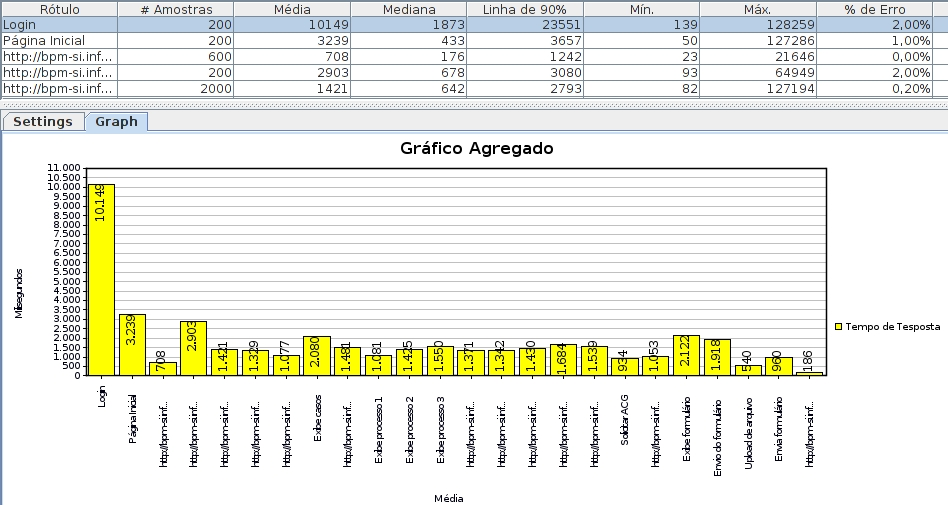
\includegraphics[width=.99\textwidth]{imagens/grafico200.jpg}
\caption{Resultado dos testes de carga com 200 usuários no JMeter.}
\label{fig:carga200}
\end{figure}



\section{Testes Funcionais}


%-Selenium
%\subsection{Seleção de Ferramentas}
Com a rápida evolução dos sistemas e tecnologias baseados na Web, o teste funcional automatizado neste ambiente tem sido alvo de avanços e também desafios, diante da grande quantidade de tecnologias envolvidas. A ideia geral de ferramentas para este ambiente é automatizar as ações de um navegador Web real ou emulado, como se fossem produzidas pelo usuário final. Dentre algumas ferramentas com esse propósito, pode-se citar iMacros, Ranorex e SilkTest, que são software proprietário; e Selenium, Watir e Sahi Open Source, que são software de código aberto e distribuídas gratuitamente.


Por motivos semelhantes aos descritos na Seção \ref{s:loadtools}, escolheu-se a ferramenta Selenium. Esta ferramenta possui basicamente duas partes complementares: Selenium IDE e Selenium WebDriver. A primeira é um plugin para o navegador Firefox, capaz de registrar e reproduzir interações do usuário com o navegador, assim permitindo criar scripts de teste rapidamente, sem escrita de código. A segunda é basicamente uma coleção de bibliotecas que, juntas, permitem escrever programas capazes de dirigir o navegador, fazendo-o se comportar como se um usuário o estivesse utilizando. A forma mais simples de utilizar o Selenium é, portanto, via o plugin para o navegador. Após gravar a execução de uma atividade no sistema, pode-se não só reproduzi-lo, mas também exportar o script para uma linguagem específica e, assim, fazer uso do WebDriver.




%o Selenium. O Selenium  é um projeto open-source e um plugin para navegadores, originalmente desenvolvido pela ThoughtWorks e possui uma comunidade ativa de desenvolvedores e usuários. Ele possui ferramentas para automatização de testes para aplicações web em múltiplas plataformas, ferramenta também permite gravação e execução de testes sem a necessidade de aprender uma linguagem específica para implementar os testes.


\subsection{Descrição dos Testes}


Em testes funcionais, é necessário considerar quais funções o sistema deve desempenhar. Além disso, é importante criar dados de entrada e determinar as saídas correspondentes. Após a execução do teste, deve-se poder comparar os resultados obtidos com os esperados. No que diz respeito às funções da aplicação BPM em questão, pode-se dizer que são todas relacionadas à execução de instâncias de um mesmo processo. No entanto, há que se considerar que o processo possui muitos fluxos dependentes dos dados de entrada.


Utilizando-se o Selenium IDE, registrou-se dados e ações para compor os testes funcionais. Na figura \ref{fig:capturaselenium}, é possível visualizar a captura da execução no navegador. O formulário na metade direita da figura corresponde ao início do processo, em que o aluno preenche sua solicitação. Nota-se que a ferramenta permite testar diversos tipos de campos HTML (seleção, campo de texto, entre outros), o que é um ponto forte. Durante o teste, é possível verificar se todas as ações foram executadas conforme esperado.




\begin{figure}[ht]
\centering
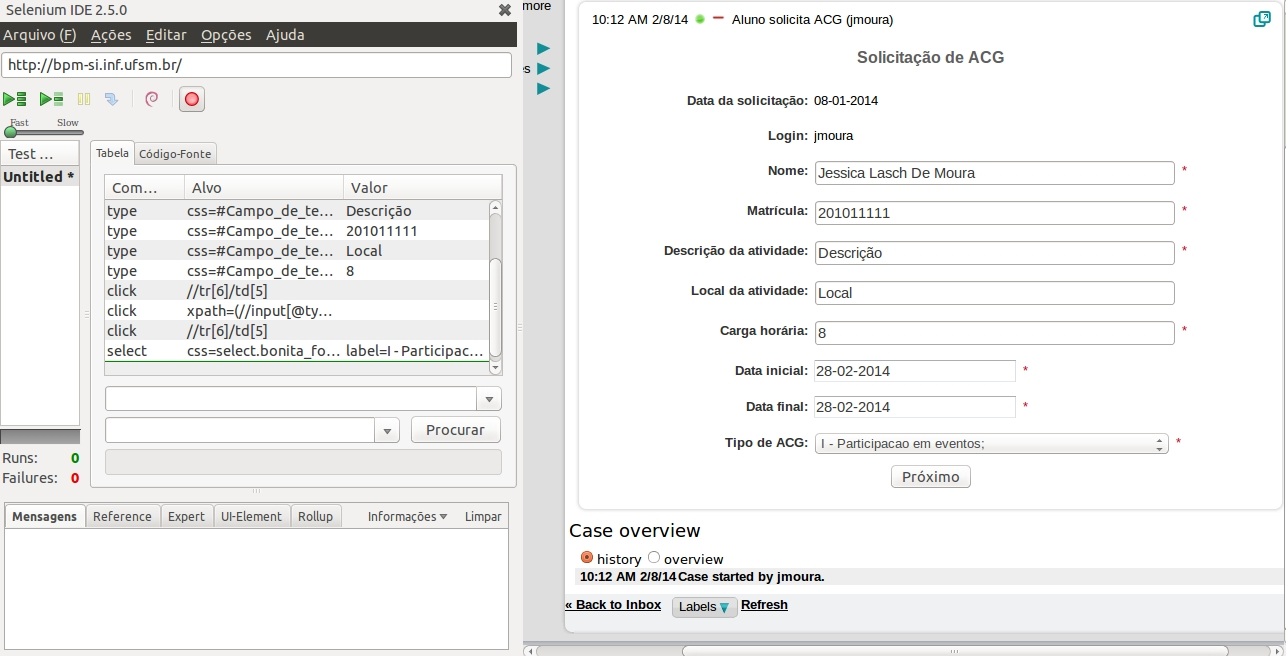
\includegraphics[width=.99\textwidth]{imagens/capturaselenium.jpg}
\caption{Captura de dados e ações através do Selenium no navegador.}
\label{fig:capturaselenium}
\end{figure}


Considerando que o processo possui muitos fluxos, todos necessários para o correto funcionamento do sistema, foram criados vários casos de teste, para diferentes papéis de usuários, com dados de entrada que levavam a caminhos distintos. Neste ponto, a criação dos testes tornou-se bastante trabalhosa, mesmo com o Selenium IDE, pois cada caso foi configurado manualmente.


O Selenium WebDriver é a alternativa para uma automatização mais completa dos testes. Um uso típico desta solução consiste em exportar um script de teste criado no Selenium IDE em uma linguagem/formato conveniente, por exemplo Java/JUnit. A partir disso, é necessário customizar o programa resultante e ligá-lo às bibliotecas do Selenium para, então, executar os testes.


Esta alternativa começou a ser explorada na aplicação de BPM em questão, quando notou-se que a abordagem possui vários pontos fracos no contexto considerado e, por isso, não foi aprofundada. Diferentemente das dificuldades técnicas encontradas nos testes de carga, encontrou-se limitações mais fundamentais. Isso é discutido na Seção a seguir.


%resultados que podem ser obtidos e
\subsection{Resultados}

Com o Selenium IDE, conseguiu-se facilmente criar testes com preenchimento automático dos formulários, passando por diferentes fluxos do processo. Os testes puderam ser reproduzidos e ações que eventualmente falharam puderam ser prontamente identificadas. Isso constituiu um avanço em relação aos testes manuais. De fato, à época do desenvolvimento da aplicação, a cada pequena modificação feita no processo como, por exemplo, adicionar ou alterar um campo num formulário, era necessário percorrer o fluxo do processo até chegar à atividade alterada. Realizar essa tarefa manualmente ocasionava um grande gasto de tempo e também era propenso a falhas humanas. Com o Selenium, parte desse tempo teria sido poupado.

Uma aplicação baseada em BPM possui diversas particularidades que tornam-se limitações para a realização do teste com o Selenium como, diferente de outros tipos de aplicações, como foi citado anteriormente, o processo possui diferentes fluxos que podem ser seguidos para chegar ao final porém, cada etapa desses fluxos pode ser realizada por um usuário diferente cumprindo um papel diferente. Com isso, para realizar o teste com o Selenium, seria necessário criar um usuário para executar cada etapa e então efetuar login, realizar a tarefa, e assim até o fim do processo. Assim, a criação do teste a ser executado se torna trabalhosa e complexa, diferente de outros tipos de sistemas onde, usualmente, efetuar o teste em uma etapa é suficiente como, por exemplo, um sistema de cadastros.

Outra limitação encontrada, foi que os dados de entrada tiveram que ser criados manualmente no Selenium IDE. Assim, tornou-se trabalhoso testar muitas combinações de entrada e também há casos que ocorreram durante a execução do sistema como nomes com caracteres especiais, por exemplo, em que depende-se de que o desenvolvedor crie esse caso específico para ser testado, nesse caso a ferramenta não oferece um auxílio em prever estes tipos de testes. Outro ponto fraco é que a comparação das entradas com as saídas esperadas não é orientada a dados, mas sim a ações (visualiza-se facilmente as ações que falham, mas não se compara facilmente os dados obtidos/esperados na saída). Além disso, foi inviável criar casos de teste manualmente para muitos fluxos do processo. Isso poderia ser contornado usando-se o Selenium WebDriver, mas estimou-se que seria necessário um tempo considerável para escrever um programa capaz de testar muitas combinações relevantes. Para testes funcionais mais completos, acredita-se que seria necessário rever a própria abordagem de desenvolvimento da aplicação. Desta forma, pode-se dizer que os testes não atingiram plenamente os objetivos.


%\section{Trabalhos Relacionados}
%outros casos semelhantes:
%artigos que usaram -JMeter,

%O teste de software voltado especificamente a aplicações de BPM é um assunto que pode ser considerado ainda em aberto. Atualmente, muitos trabalhos de pesquisa têm focado em etapas de monitoramento e otimização em BPM~\cite{Gambini:2011:AEC:2040283.2040300, Liu:2011:BAM:2040283.2040307, deLeoni:2012:AEL:2413516.2413525, Ramezani:2012:DIM:2413516.2413545}, que são etapas dedicadas a identificar e corrigir problemas. Embora exista alguma relação com testes em BPM, tratam-se geralmente de abordagens mais voltadas a aspectos de gestão, não de software . Por outro lado, um assunto que tem sido bastante abordado é o teste automatizado de aplicações orientadas a serviços Web~\cite{soatest2008}. Embora se trate de um nicho de teste de software, e mesmo que haja uma relação entre BPMS e serviços Web, acredita-se que esta abordagem não abarque toda a problemática do teste de aplicações de BPM. Na aplicação alvo deste trabalho, em particular, a abordagem orientada a serviços Web não poderia ser usada, pois o BPMS empregado baseia-se numa arquitetura que não expõe seus serviços.


%No que diz respeito a relatos de experiência e estudos de caso, costuma haver espaço para isso em conferências internacionais sobre BPM e engenharia de software. Conforme van der Aalst (2013), em uma análise de várias edições da International Conference on Business Process Management, há muitos artigos que descrevem esforços de implementação e estudos de caso. No entanto, vários deles envolvem software que não é disponível ao leitor ou casos que são deliberadamente vagos~\cite{aalst2013survey}. No Brasil, conferências como o Simpósio Brasileiro de Sistemas de Informação e o Simpósio Brasileiro de Engenharia de Software incluem BPM e testes de software entre seus tópicos de interesse mas, até onde foi possível verificar, ainda não foram publicados trabalhos associando esses dois tópicos.

%Monitoramento: Business Artifact-Centric Modeling for Real-Time Performance Monitoring
%Verificação:
%Aligning Event Logs and Declarative Process Models for Conformance Checking.
%Massimiliano De Leoni, Fabrizio Maria Maggi and Wil van der Aalst
%Context-Aware Compliance Checking.
%Jan Martijn Van Der Werf, Eric Verbeek and Wil Van Der Aalst
%Where Did I Misbehave? Diagnostic Information in Compliance ...




%Embora o termo ``teste'' não seja frequente na literatura sobre BPM, o ciclo de vida de aplicações de BPM inclui as etapas de monitoramento e otimização, que se dedicam a identificar e corrigir problemas~\cite{weske}. Tal visão do ciclo de vida é comumente voltada a aspectos de gestão, não de tecnologia (software). Mesmo assim, acreditamos que o teste de software relacione-se particularmente com essas etapas e, de forma geral, possa contribuir significativamente para o sucesso de aplicações de BPM.


%O artigo 'Um estudo sobre testes de desempenho com aplicação prática utilizando a ferramenta JMeter' (referencia) descreve o resultado de um estudo sobre testes de desempenho aplicado teste de desempenho aplicado em uma arquitetura e-commerce hipotética utilizando o JMeter. Diferentemente do presente trabalho, este artigo não possui usuários e um sistema real para ser analisado, sendo seu o objetivo analisar os dados para o desenvolvimento de um aplicativo, não para a melhoria do sistema.


%selenium e JMeter
%No trabalho “A Test Automation Framework Based on Web” \cite{wang2012test} é relatada a criação de um framework para teste automatizado de aplicações web, utilizando as ferramentas Selenium e JMeter. Os resultados do trabalho demonstram que as ferramentas ajudam, bem como o framework, ajudam a melhorar a qualidade do software e a aumentar a eficiência do desenvolvimento.


%testes com Selenium;
%O artigo “Automating functional tests using Selenium”\cite{holmes2006automating} é um relato de experiência utilizando o Selenium para testes automatizados e descreve as dificuldades e aprendizados com esta ferramenta, como tempo para escrever os scripts de teste bem como integração. Entretanto, os testes são baseados em aplicações Web simples e não em BPM. De fato não foram encontrados artigos que unissem BPM e a ferramenta Selenium para testar processos.


%trabalhos mais teoricos sobre teste de BPM (possivelmente citar na Seção 2)
%No white-paper “Performance Testing of Business Process Management (BPM) aplications using JMeter” \cite{} é um artigo teórico que defende a importância do teste de performance nas aplicações baseadas em BPM, para evitar a falha dos processos no ambiente de produção, bem como defende o uso do JMeter para implementar os testes levantando várias justificativas, dentre elas o fato de ser uma ferramenta gratuita que tem tantas funcionalidades quanto ferramentas pagas. Diferente do nosso trabalho, este não possui um ambiente em produção ou um processo real, com problemas reais, para efetuar o teste com o JMeter. O trabalho apenas trata da importância dos testes e sobre a potencialidade do JMeter.




%
%-artigos que fizeram teste de BPM
%http://www.pushtotest.com/business-process-management-bpm-testing
%http://pt.slideshare.net/samarin/bpm-context-for-testing-presentation
%http://www.tcs.com/SiteCollectionDocuments/Brochures/Assurance-Brochure-BPM-Automated-%Test-Solution-0613-1.pdf <- empresa, solucao paga


%Tipicamente, aplicações de BPM envolvem usuários com múltiplos papéis e o fluxo de execução possui muitos caminhos possíveis. Isso contrasta com um comportamento comumente observado em aplicações Web tradicionais, com poucos papéis (geralmente, usuário e administrador) e poucos caminhos possíveis (muitas vezes, sem desvios condicionais).



\section{Conclusão}


Neste trabalho, foram conduzidas experiências de teste de software em uma aplicação real de BPM, que encontra-se implantada em uma instituição pública de ensino. Na delimitação o trabalho, focou-se em dois tipos de teste: testes de carga e testes funcionais. Na indisponibilidade de ferramentas específicas para o teste de aplicações de BPM, buscou-se selecionar ferramentas consagradas na área de teste de software.


As experiências de testes de carga mostraram que uma ferramenta típica para este propósito (Apache JMeter), mesmo não sendo integrada ao BPMS, tornou possível atingir os objetivos dos testes. Em particular, conseguiu-se determinar um nível de carga em que o tempo de resposta seria muito alto para os usuários da aplicação de BPM.


Por outro lado, os testes funcionais, mesmo utilizando uma ferramenta popular (Selenium), não atingiram plenamente os objetivos. Esses resultados sugerem que a automação deste tipo de teste não seja uma tarefa trivial em aplicações de BPM, principalmente pela falta de ferramentas adequadas e alinhadas com o ciclo de vida de BPM.


Embora as experiências não tenham sido exaustivas, acredita-se que constituam uma contribuição para profissionais e pesquisadores interessados dedicados aos tópicos de BPM e teste de software. Como trabalhos futuros, pode-se destacar a exploração de ferramentas de geração de casos de teste, na hipótese de que possam ajudar a alinhar os testes com as saídas e entradas do processo. Outra via que merece ser explorada são os testes de regressão, para auxiliar a encontrar possíveis problemas após alterações no processo, que podem ser frequentes dependendo do caso.




\bibliographystyle{sbc}
\bibliography{sbc-template}


\end{document}





